\chapter{Introduction}\label{ch:intro}
The Large Hadron Collider (LHC) is the world's largest and most powerful particle collider. It was built by the European Organization for Nuclear Research (CERN) between 1998 and 2008. From the early 2010 up until today it has produced several proton run yielding a great amount of data gathered by the four main experiments (CMS, ATLAS, ALICE and LHCB). The data allowed for the publication of hundreds of articles and between those one of the most important: the experimental confirmation of the Higgs Boson existence.\\ The current configuration of LHC will remain substantially unvaried until 2023 when, during the Long Shutdown 3 (LS3), several upgrades of the accelerator, will allow a significant increase of the instantaneous luminosity delivered. The upgraded version of the collider is referred to as High Luminosity Large Hadron Collider (HL-LHC).

\section{HL-LHC}
It is expected that by 2023 the quadrupoles magnet that focus the proton beans of LHC for the two biggest experiment (CMS and ATLAS) will be close to the end of their life cycle due to radiation exposure. The substitution of those quadrupoles and the addition of new upgrades to optimize the bunch overlap at the interaction region, will result in a significant increase of the delivered luminosity.
The proposed operating scenario is to have $5 \times 10^{34} \unit{cm^{-2}s^{-1}}$ of instantaneous luminosity, roughly five times more than the current one.\\
As a direct consequence of the increase in luminosity a high number of events happening during the same bunch crossing is expected, this phenomenon is often referred to as \textit{pileup}.\\
It is expected that an average of 140 pileup events \cite{tdr} per bunch crossing will take place as a result of the upgrade to LHC, up to spikes of 200 (while at the time of the writing the average is 22). All the main experiments will need to upgrade their detectors in order to solve the tracks originating from so many verteces and also in order to replace the components damaged by ten years of radiations with new ones able to sustain ten more years of even higher radiation.\\
As we developed this work within the CMS collaboration we focus here on the upgrades of that experiment only.

\section{CMS Phase-II upgrade}
\begin{figure}
\centerline{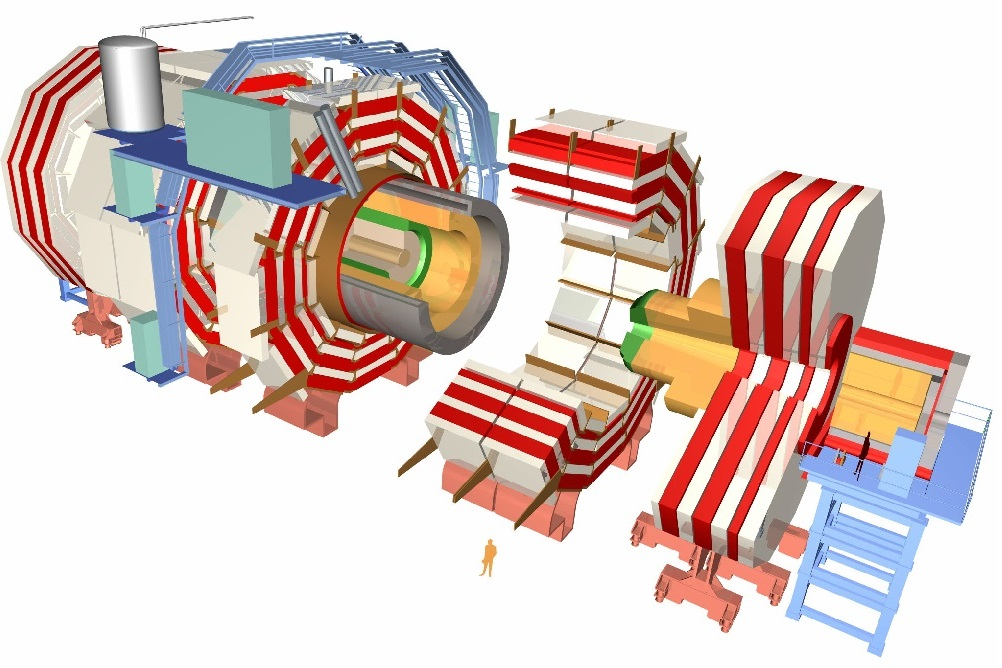
\includegraphics[width=0.8\textwidth]{intro/cms.jpg}}
\caption{An exploded view of the CMS detector in its current configuration.}
\label{cms}
\end{figure}

The Compact Muon Solenoid (CMS) is an hermetic particle detector gathering data from LHC collisions. Its general design consists of a cylinder parallel to the beam lines, called \textit{Barrel} and two discs, called \textit{EndCaps}, closing the cylinder at both ends, perpendicular to the beam lines.\\
The barrel is actually made of a series of cylindrical sub-detector each one enclosing the smaller detectors closer to the beam line. Starting from the innermost detector there is the silicon pixel tracker, followed by the silicon strips tracker. Around the tracker lies the Electromagnetic Calorimeter (ECAL), made of Lead-Tungsten crystals and followed by the Hadronic Calorimeter (HCAL) featuring brass plates interleaved by plastic scintillators. The superconducting solenoid encloses all the above and provides an inner magnetic field of 3.8 Tesla. The outermost cylinder is the one hosting the muon chambers placed between the steel return yoke that also allows the external magnetic field lines to be parallel to the beam lines and uniform. The endcaps features a similar sequence of sub-detector organized in discs of increasing radius. A detailed description of the CMS detector is given in reference \cite{cms}.\\

Following we will give a brief overview of the upgrades proposed for CMS to comply with the predicted conditions of \textit{Phase II}.

\begin{itemize}
\item \textbf{Tracker} By the time LS3 will begin, the tracker, the barrel part and the endcaps parts, will suffer significant radiation damage -especially being the first material to be irradiated by the collisions products- and must be completely replaced. To maintain adequate track reconstructions capabilities at the conditions of HL-LHC the granularity of all the elements of the sub-detector will be increased by roughly a factor four.
\item \textbf{Calorimeter Endcaps} The forward regions of a collider detector receive the most radiation. Therefore by LS3 the Calorimeters Endcaps will also need replacement. The new calorimeter is called High Granularity Calorimiter (HGCAL) and has electromagnetic and hadronic sections with excellent segmentation. It is a sampling calorimeter where the active layers of silicon detectors are interleaved with copper and tungsten plates.
\item \textbf{Muon Endcaps} The forward muon system will receive additional chambers to maintain a good trigger acceptance. A combination of Gas Electron Multiplier and and Resistive Plate Chambers will be installed to increase the performance of the overall muon system.
\item \textbf{Low and High Level Triggers} The hardware trigger, also called Level 1, will be improved by upgrading the readout electronics in some of the sub-detectors that will be kept for Phase-II. Thus the hardware trigger rate will increase from the current 100 $\unit{kHz}$ to the 750 $\unit{kHz}$ needed for the peak 200 events pileup predicted for Phase-II. Also the software trigger: called High Level Trigger (HLT), that is the one taking into account the information of multiple sub-detectors for each event, will need to be upgraded to keep up with the increase in data rate. It is predicted that the computational power today dedicated to the HLT will need to increase up to a factor of 12.
\end{itemize}

In this work we are particularly interested by the new calorimeters endcaps, HGCAL, and the effect that the new design will have on the online reconstruction performed by the High Level Trigger. As the major difference with respect to the current sub-detector is the part dedicated to the electromagnetic detection, that is the part we mainly focus our work on.

\section{The High Granularity Calorimeter}
As mentioned above the Electromagnetic part of the HGCAL is a sampling calorimeter where layers of silicon detectors are interleaved by absorber of Tungsten-Copper.
The calorimetry usually express the thickness of the materials traversed by the electromagnetic radiations in terms of their \textit{radiation length}, denoted $X_0$, which is the mean path length required to reduce the energy of relativistic charged particles by a factor $1/\mathrm {e}$. The calorimeter is then composed of 28 layers each having an absorber and a plane of silicon detector. In details the thickness of the layers, in order from inward to outward, are as follow:
\begin{itemize}
\item 10 layers: 0.65 $X_0$
\item 10 layers: 0.88 $X_0$
\item 8 layers: 1.26 $X_0$
\end{itemize}
Resulting in a total length of 26 $X_0$.\\
The modules are shaped as two adjacent hexagons as shown in Figure \ref{hgcalMod}, they will be mounted in several copper and tungsten absorber ``petals'' which in turns will be inserted in the ``cassettes'' of the final carbon fiber structure, Figure \ref{hgcalStruct}.

\begin{figure}
\centerline{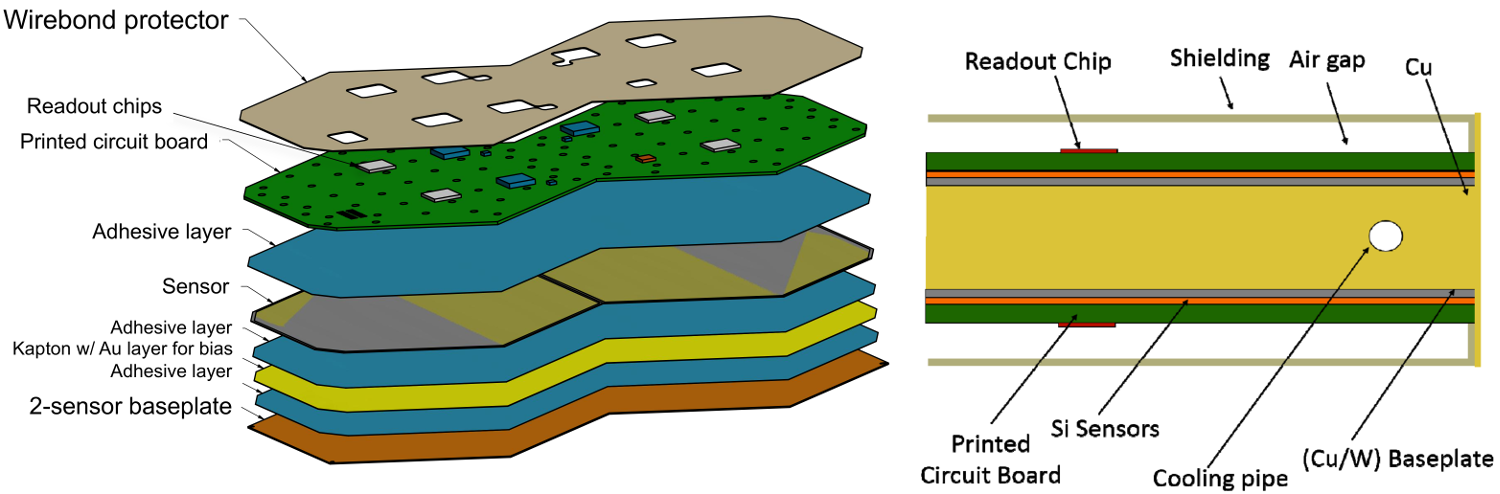
\includegraphics[width=0.8\textwidth]{intro/hgcalMod.png}}
\caption{(Left) A module of HGCAL, consisting of printed circuit board, silicon sensor and absorber. (Right) Two modules mounted on either sides of a copper tungsten absorber also used for the cooling of the system.}
\label{hgcalMod}
\end{figure}

\begin{figure}
\centerline{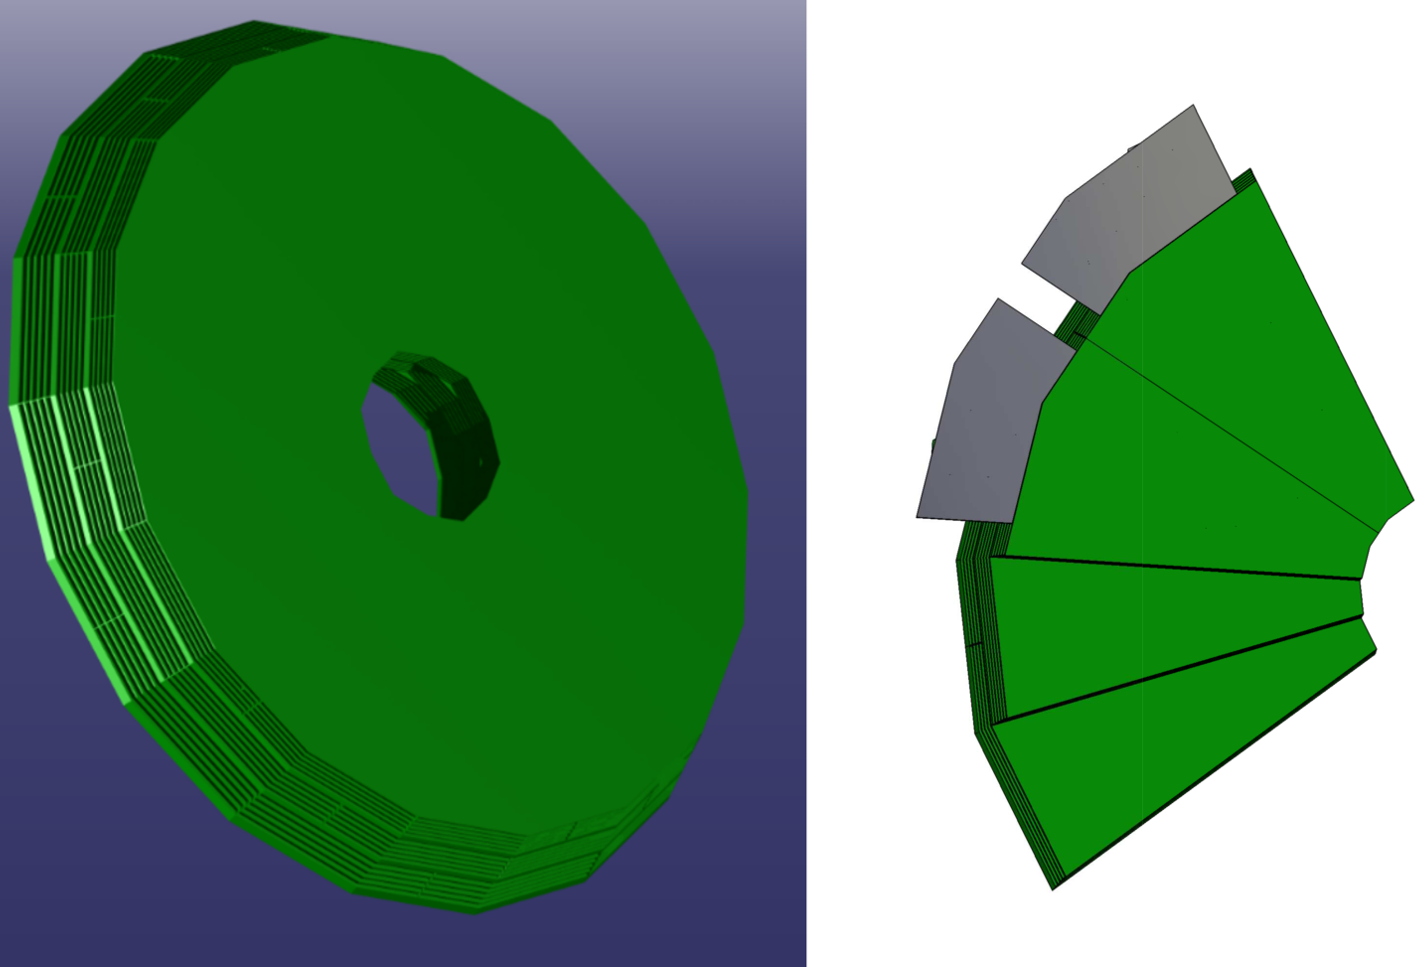
\includegraphics[width=0.8\textwidth]{intro/hgcalStruct.png}}
\caption{(Left) The final Electromagnetic HGCAL endcap carbon-fiber structure. (Right) The petals inserted into the slots of the structure.}
\label{hgcalStruct}
\end{figure}

The modules have an active area of 1.05 $\unit{cm^2}$ or 0.53 $\unit{cm^2}$ depending on their position in the endcap. Totally approximately 22000 modules will constitute the calorimeter providing a total area of active silicon of 320 $\unit{m^2}$ that will be read out by 4.3 million channels.\\


\section{Calorimeter reconstruction}\label{sec:hgcal_clustering}
Following we describe how the electromagnetic particles interacts in an electromagnetic calorimeter and how this interaction is exploited to best detects the properties of the radiation. We describe also how the readout electronics of the calorimeter interprets the signals coming for the detectors and lastly how the reconstruction software can piece together those information to evaluate the direction and the energy of the incoming particle.

\subsection{The electromagnetic shower}
When a photon enter a material three possible interactions can take place, depending on its energy:
\begin{itemize}
\item \textbf{Photoelectric effect} The photon interacts with an atom of the material if its energy is greater than the binding energy of one of the atom's electron. The photon is absobed and an electron is scattered off the atom with the same energy of the incoming photon.
\item \textbf{Compton scattering} Inside the electromagnetic field of an atom the photon scatters with one of the electrons of the atom. The photon loses a fraction of energy which is transferred to the emitted electron.
\item \textbf{Pair production} When the photon is highly energetic and passes by the nucleus of an atom a pair production can occur. The incoming photon interacts with the Coulomb field of the nucleus of the atom and is absorbed creating a pair electron-positron that shares the initial energy of the photon.
\end{itemize}

It is important to note that all the above interactions produces one or more electrons at the expense of the initial energy of the photon.
When it is an electron to enter a material the possible interactions are somewhat similar:
\begin{itemize}
\item \textbf{Ionization} The incoming electron scatters off another electron of the atoms, leaving the atom ionizied. The incoming electron loses some energy transferred to the electron emitted by the atom.
\item \textbf{Bremsstrahlung} ``Braking radiation'' from the German. It occurs when a high energy electron interacts with the Coulomb field of the nucleus of an atom. The incoming electron is slowed by the electric attraction of the nucleus and this decelleration causes the electron to emit a photon.
\item \textbf{Cherenkov radiation} When a charged particle passes through a dielectric material at a speed greater than the phase velocity of the light in that material a characteristic radiation is emitted. 
\end{itemize}

Again note that the above described interactions results in the production of one or more photons.\\

The net effect of an electron or a photon interacting with some materials is therefore a chain reaction that results in splitting the initial energy of the incoming particle in more photons and electrons of increasingly smaller energy, until their energy is too low to generate more interactions.
The development of this chain reaction is named \textit{electromagnetic shower} because while generating more particles those scatters off in a slight different direction respect the original particle. Therefore the shower transverse size -that perpendicular to the original particle- gets bigger and bigger until it stops. The final size of the shower is determined by the \textit{Molière radius} which is a property of the material and is such that $90\%$ of the electromagnetic shower is contained in a cylinder of one Molière radius.

\subsection{HGCAL digitization}
The silicon pad of the Calorimeter modules can only detect the transit of a charged particle. Over a well developed electromagnetic shower on average 2/3 of all particles will be electrons and positrons, while the rest 1/3 photons that are not detected. By knowing this fraction and by measuring the electrons energy deposit on the silicon pads a calibration is therefore possible to allow the reconstruction of the total energy of the original particle entering the calorimeter.\\
In the CMS terminology when a pad reveal a signal above the signal threshold gets recorded and takes the name of \textit{rechit} (as Reconstructed Hit). A rechit keeps the information of the identifier of the pad that revealed the signal, the absolute position of the hit in the CMS coordinate system and the energy measured.\\
Since the Molière radius of the shower depends on the $X_0$ thickness of material traversed, the size of the shower grows while traversing the layers of HGCAL. A simulation study has been performed to evaluate the Molière radius variation with respect to the layers of the calorimeter. Figure \ref{moliereHgcal} shows the result of the study.\\

\begin{figure}
\centerline{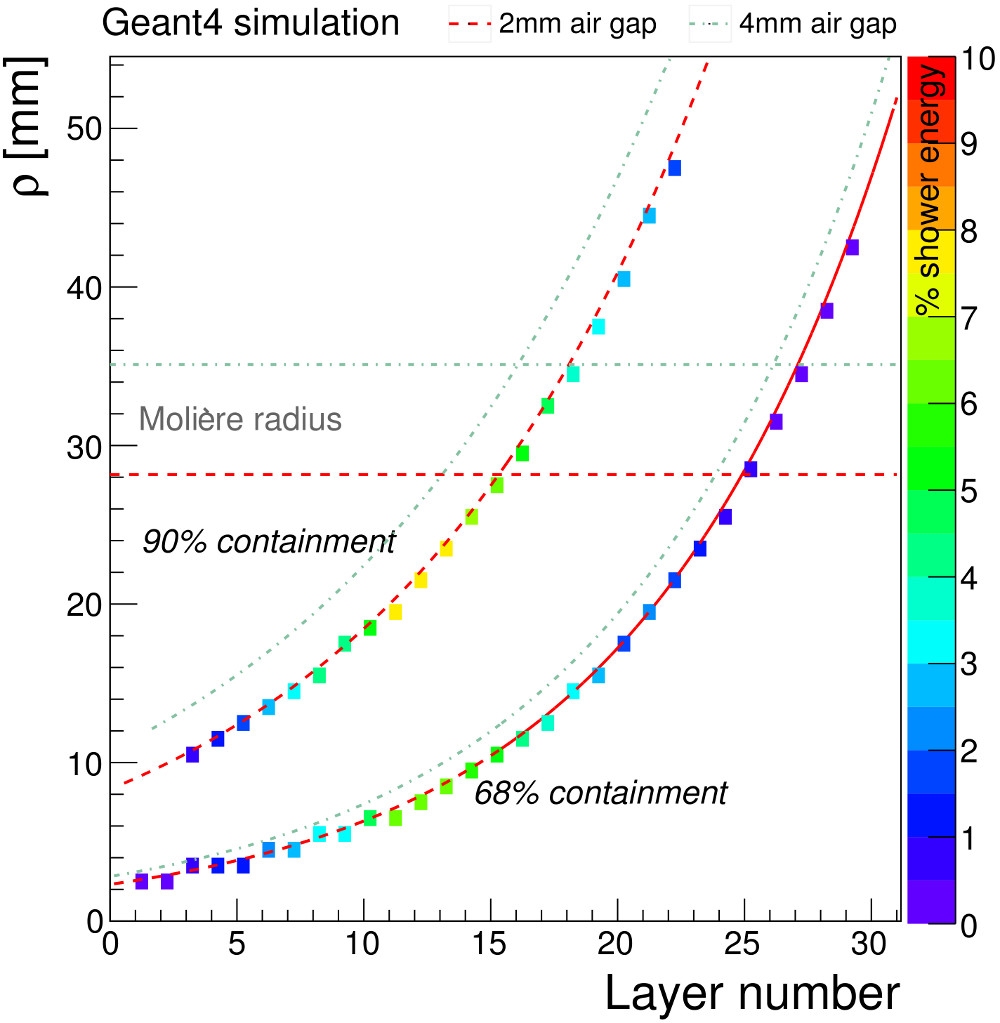
\includegraphics[width=0.8\textwidth]{intro/moliereHgcal.png}}
\caption{Molière radii, $\rho$, containing $68\%$ and $90\%$ of the energy deposited in a single layer by a shower, as a function of the silicon layer. The colour-coded rectangles indicate
the fraction of total energy deposited inside the $68\%$ and $90\%$ containment radii of each layer.}
\label{moliereHgcal}
\end{figure}
\clearpage

We can now use the information of the maximum Molière radius ($6.0 \unit{cm}$) and the minimum silicon pad size ($0.53 \unit{cm^2}$) to evaluate the maximum number of rechits recorded in a given layer for a given shower. This quantity will be useful later when discussing the algorithm used to perform the reconstruction.\\
We want to be conservative and consider the energy deposited in two Molière radii, which correspond to $95\%$ of the shower. The maxium number of possible rechits in a square of side $2 \times \rho_m$ in the modules where the pads have the smallest area is then: $(6.0 \unit{cm} * 2)^2/0.53 \unit{cm^2} \simeq 273$.

\subsection{Clusterization}
A critical step in the reconstruction of the calorimeter electromagnetic shower is the \textit{clusterization}, that is the procedure by which the groups of rechits belonging to the same shower are identified.\\
There are many known, and some very complex, clustering algorithms, however, in the case of a calorimetric shower the information on the Molière radius is a very powerfull one as it limits \textit{a priori} the area where to find all the rechits belonging to a given initial particle.\\
Throughout this work we implent a clustering algorithm based on the above principle: for each rechit found in the calorimeter we search for all its \textit{nearest neighbors} rechits lying in a square of two Molière radii centered around the rechit for which we search the neighbors.\\
Although it might seem a very simple algorithm, the simulation of the Phase II conditions along with the very high granularity of the HGCAL shows that the number of rechits per events that will be necessary to process can be as high as $3 \times 10^5$ and more. We will show on this work how a simple algorithm would not be sufficient to perform an all nearest neighbors search of so many points in a reasonable amount of time.

\subsection{Reconstruction}
Once the cluster in each layer of the calorimeter are built, the reconstruction software can proceed in \textit{linking} them. There are several different technique to achieve the linking of the cluster. A simple, yet effective, one consists in searching the clusters of the different layers inside a cone centered in the interaction point of CMS and linking one by one starting from the inner layer to the next one and when more than one cluster is present in the next layer the one with the minimal distance is chosen.\\
Once all the clusters are linked togheter their total energy and the direction of the incoming particle can be evaluated.

\section{HLT and computation challanges}
It is forseen that the Level 1 trigger will need to operate five times faster than the current one, that is at $500 \unit{kHz}$. It is also expected that the L1 trigger will maintain its current rejection factor of roughly a 100. The High Level Trigger is, therefore, expected to operate at $5 \unit{kHz}$, which means that the events will have to be processed at $0.2 \unit{ms}$.\\
This time constraint will pose an extremely hard challange for the clusterization of the HGCAL rechits. This is the reason of this work, that aims to tackle the challange through the use of what is currently new technology, and hardware, that is expected to greatly increase its performance in the years to come before the Long Shutdown 3.

